\documentclass[]{article}
\usepackage{graphicx}
\usepackage{amsmath}
\usepackage{graphics}
\usepackage{latexsym}
\usepackage{amssymb}
\usepackage{graphics}
\usepackage{color}
\usepackage{subfigure}
\usepackage{wrapfig}

\title{Algorithm Notes for Merge Tree Computation}
\author{Peer-Timo Bremer}
\date{}

\begin{document}
\maketitle

\section{Concepts}

Some random thoughts

\begin{itemize}
\item There exist several different {\it indices} by which we can identify vertices :\\
  (1) the global order defined by the global mesh\\
  (2) the block order defined by a regular subset of the data\\
  (3) the local order defined as compact order of pre-filtered vertices
\end{itemize}

\section{Current Single Core Streaming Algorithm}
\begin{figure*}[htbp]
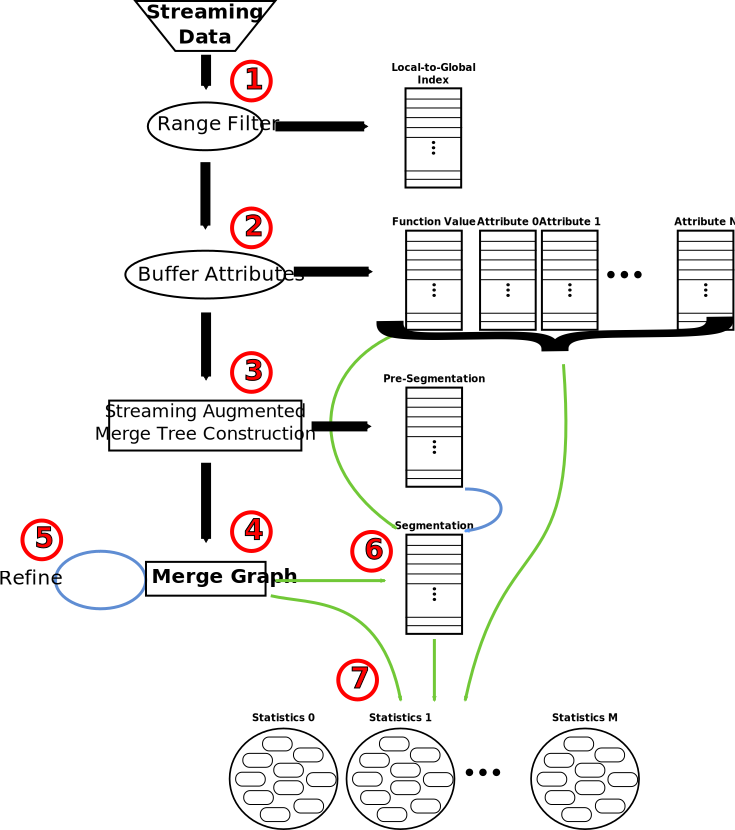
\includegraphics[width=\linewidth]{MergeTree_Outline}\label{fig:ridge-valley}
\caption{Single core streaming algorithm outline.}
\end{figure*}

\paragraph{Input.} 

\begin{itemize}
\item Sequence of {\it vertices}, $v_i$, {\it edges}, $e_j$, and {\it
    finalization info}, $f_i$.
\item Each vertex contains a global index and $k > 0$ coordinates of which the
  first one is used as function.
\item Each edge contains two global indices
\item Each finalization info contains one global index
\end{itemize}

\paragraph{Output.}

\begin{itemize}
\item Potentially refined {\it merge tree}
\item Segmentation in local order
\item Global indices in local lorder
\end{itemize}

\paragraph{Steps.}

\begin{enumerate}
\item Parse the data and filter based on a function range. This implicitly
  creates a new order of vertices. The original vertex ids are stored for later
  drawing.\\
  {\it Needs and index map from global to local index space to adjust edge
    indices}
\item Buffer the function value and all attributes that are needed for
  statistics for all vertices that have passed the filterw. Create minimal vertex
  token $(id,function)$.
\item Streaming construction of the merge tree. Each time a vertex is removed
  from memory record its last segmentation index.\\
  {\it Needs the local, compact index space for dense storage}
\item Collect the nodes and arcs as they are finalized from the construction
  algorith.\\
  {\it Nodes are identified in the local index space.}
\item Refine the graph to shorten overly long arcs. This is done in place, New
  nodes will be marked as not belonging to the orginal mesh (they are {\it
    virtual}.
\item Correct the pre-segmentation in place using a path-compression type
  lookup. \\
  {\it Each segmentation id corresponds to a vertex id. We must be able to find
    the corresponding vertex in the array (trivial in the local index space).}
\item Collect the attributes of all vertices into sets of statitics one for each
  feature / node
{\it Needs a map from feature / node id to a compact representation}
\end{enumerate}


\end{document}